% Copyright 2016 - 2018 Bas van Meerten and Wouter Franssen
%
%This file is part of ssNake.
%
%ssNake is free software: you can redistribute it and/or modify
%it under the terms of the GNU General Public License as published by
%the Free Software Foundation, either version 3 of the License, or
%(at your option) any later version.
%
%ssNake is distributed in the hope that it will be useful,
%but WITHOUT ANY WARRANTY; without even the implied warranty of
%MERCHANTABILITY or FITNESS FOR A PARTICULAR PURPOSE.  See the
%GNU General Public License for more details.
%
%You should have received a copy of the GNU General Public License
%along with ssNake. If not, see <http://www.gnu.org/licenses/>.

\documentclass[11pt,a4paper]{article}
% Copyright 2016 - 2017 Bas van Meerten and Wouter Franssen
%
%This file is part of ssNake.
%
%ssNake is free software: you can redistribute it and/or modify
%it under the terms of the GNU General Public License as published by
%the Free Software Foundation, either version 3 of the License, or
%(at your option) any later version.
%
%ssNake is distributed in the hope that it will be useful,
%but WITHOUT ANY WARRANTY; without even the implied warranty of
%MERCHANTABILITY or FITNESS FOR A PARTICULAR PURPOSE.  See the
%GNU General Public License for more details.
%
%You should have received a copy of the GNU General Public License
%along with ssNake. If not, see <http://www.gnu.org/licenses/>.

\usepackage[british]{babel}
\usepackage{graphicx,booktabs,listings,amsmath,pgfplots,pgfplotstable}
\usepackage[small,bf,nooneline]{caption}
\usepackage{subcaption}
\usepackage[sort&compress,numbers]{natbib}
\usepackage{tikz}
\usepackage{mathtools}
\usepackage[nottoc]{tocbibind}%adds bibliography to table of contents.
\graphicspath{{./images/}}
%\setlength{\textwidth}{453pt} %597 pt is the a4 paperwidth. Minus 2 in margin. 72 pt = 1 in
%\setlength{\hoffset}{-\oddsidemargin}
%\setlength{\voffset}{-30pt} %
%\setlength{\textheight}{651 pt} %a4 height 845 pt minus 2* total headheight. In this case 2*88pt
%% examine margines via the layout package. Use command \layout{} in document to draw a picture.
%\setlength{\parindent}{0.5 cm}
%\setlength{\parskip}{0 cm}
\usepackage[left=82pt,right=82pt,top=95pt,bottom=95pt,footnotesep=0.5cm]{geometry}
%\setlength{\headheight}{14pt}

%define colours--------------------
%dark
\usepackage{xcolor}
\definecolor{MyGrayD}{RGB}{1,1,1}
\definecolor{MyRedD}{RGB}{237,45,46}
\definecolor{MyGreenD}{RGB}{0,140,71}
\definecolor{MyBlueD}{RGB}{24,89,169}
\definecolor{MyOrangeD}{RGB}{243,125,34}
\definecolor{MyPurpleD}{RGB}{102,44,145}
\definecolor{MyBrownD}{RGB}{161,29,32}
\definecolor{MyPinkD}{RGB}{179,56,147}
%normal
\definecolor{MyGray}{RGB}{114,114,114}
\definecolor{MyRed}{RGB}{241,89,95}
\definecolor{MyGreen}{RGB}{121,195,106}
\definecolor{MyBlue}{RGB}{89,154,211}
\definecolor{MyOrange}{RGB}{249,166,90}
\definecolor{MyPurple}{RGB}{158,102,171}
\definecolor{MyBrown}{RGB}{205,112,88}
\definecolor{MyPink}{RGB}{215,127,179}
%light
\definecolor{MyGrayL}{RGB}{204,204,204}
\definecolor{MyRedL}{RGB}{242,174,172}
\definecolor{MyGreenL}{RGB}{216,228,170}
\definecolor{MyBlueL}{RGB}{184,210,235}
\definecolor{MyOrangeL}{RGB}{242,209,176}
\definecolor{MyPurpleL}{RGB}{212,178,211}
\definecolor{MyBrownL}{RGB}{221,184,169}
\definecolor{MyPinkL}{RGB}{235,191,217}
%----------------------------------

%Figure ref with hyperref
\newcommand{\fref}[1]{\hyperref[#1]{Figure \ref*{#1}}}
\newcommand{\sref}[1]{\hyperref[#1]{Section \ref*{#1}}}
\newcommand{\tref}[1]{\hyperref[#1]{Table \ref*{#1}}}

%Makes a new command for figures with input values: filename, width(times linewidth),
% caption and label.
\newcommand{\onefigure}[4]{
\setlength{\captionwidth}{#2\linewidth}
\begin{figure}
\includegraphics[width=#2\linewidth]{#1}
\centering
\parbox{\linewidth}{\caption{#3}
\label{#4}}
\end{figure}
}

%Makes a new command for tikz figures with input values: tikz commands, 
% caption and label.
\newcommand{\onetikz}[3]{
\settowidth{\captionwidth}{#1}
\ifthenelse{\lengthtest{\captionwidth<0.7\linewidth}}{\setlength{\captionwidth}{0.7\linewidth}}{}

\begin{figure}
\centering
#1
\centering
\parbox{\linewidth}{\caption{#2}
\label{#3}}
\end{figure}
}

%Makes a new command for two figures next to each other with input values: filename1, caption1, label1,filename2, caption2 and label2. Figure width is set to 0.47\linewidth and the space between the figures is filled with \hfill so the sides of the figures align with to edge of the line.
\newcommand{\twofigure}[6]{
\setlength{\captionwidth}{\linewidth}
\begin{figure*}[ht!]
\begin{minipage}[t]{0.47\linewidth}
\includegraphics[width=\linewidth]{#1}
\centering
\caption{#2}
\label{#3}
\end{minipage}
\hfill
\begin{minipage}[t]{0.47\linewidth}
\centering
\includegraphics[width= \linewidth]{#4}
\centering
\caption{#5}
\label{#6}
\end{minipage}
\end{figure*}
}


%Makes a new command for a table with caption witdh equal to the total table width. Input: tabular, caption and label. Example:
%\onetable{
%\begin{tabular}{ccc}
%a&b&c\\
%\hline
%1&1&1\\
%1&1&1\\
%1&1&1\\
%\end{tabular}
%{The caption.}
%{tab:table1}
%}
\newcommand{\onetable}[3]{
\settowidth{\captionwidth}{#1}
\ifthenelse{\lengthtest{\captionwidth<0.7\linewidth}}{\setlength{\captionwidth}{0.7\linewidth}}{}
\begin{table}
\caption{#2}
\vspace{-0.24cm} %Puts caption close to toprule
\label{#3}
\centering
#1
\end{table}
}

%Makes a long table with captionwidth equal to tablewidth. It takes the following arguments:
%1: Column specifier (e.g. cccc)
%2: Caption
%3: Label
%4: First head (i.e. first row of regular table)
%5: Head of consecutive pages
%6: Foot of pagebreak
%7: Lastfoot (e.g. \midrule)
%8: Body of table
\newcommand{\onelongtable}[8]{
\begin{center}
\settowidth{\captionwidth}{
\begin{tabular}{#1}
#4
#8
\end{tabular}} % This ends the captionwidth part. Next comes the real table.

\begin{longtable}{#1}
\caption{#2}\\
\vspace{-0.74cm} %Puts caption close to toprule
\label{#3}\\

#4
\endfirsthead

#5
\endhead

#6
\endfoot

#7
\endlastfoot

#8
\end{longtable}
\end{center}}




%1:pgfplots code
%2:width
%3:caption
%4:label
\newcommand{\pgfplotsfigure}[4]{
\pgfplotsset{width=#2\linewidth}
\setlength{\captionwidth}{#2\linewidth}
\begin{figure}[t]
\centering
#1
\centering
\parbox{\linewidth}{\caption{#3}
\label{#4}}
\end{figure}
}


\usepackage[bitstream-charter]{mathdesign}
\usepackage[T1]{fontenc}
\usepackage[protrusion=true,expansion,tracking=true]{microtype}
\usepackage{siunitx}

%Set section font
\usepackage{sectsty}
\allsectionsfont{\color{black!70}\fontfamily{SourceSansPro-LF}\selectfont}
%--------------------


%Set toc fonts
\usepackage{tocloft}
%\renewcommand\cftchapfont{\fontfamily{SourceSansPro-LF}\bfseries}
\renewcommand\cfttoctitlefont{\color{black!70}\Huge\fontfamily{SourceSansPro-LF}\bfseries}
\renewcommand\cftsecfont{\fontfamily{SourceSansPro-LF}\selectfont}
%\renewcommand\cftchappagefont{\fontfamily{SourceSansPro-LF}\bfseries}
\renewcommand\cftsecpagefont{\fontfamily{SourceSansPro-LF}\selectfont}
\renewcommand\cftsubsecfont{\fontfamily{SourceSansPro-LF}\selectfont}
\renewcommand\cftsubsecpagefont{\fontfamily{SourceSansPro-LF}\selectfont}
%--------------------

%Define header/foot
%\usepackage{fancyhdr}
%\pagestyle{fancy}
%\fancyhead[LE,RO]{\fontfamily{SourceSansPro-LF}\selectfont \thepage}
%\fancyhead[LO,RE]{\fontfamily{SourceSansPro-LF}\selectfont \leftmark}
%\fancyfoot[C]{}
%--------------------

%remove page number from first chapter page
%\makeatletter
%\let\ps@plain\ps@empty
%\makeatother
%----------------------

\usepackage[hidelinks,colorlinks,allcolors=black, pdftitle={2D-PASS processing in ssNake},pdfauthor={Wouter M.J.\ Franssen}]{hyperref}

\interfootnotelinepenalty=10000 %prevents splitting of footnote over multiple pages
\linespread{1.2}

\title{\color{black}\fontfamily{SourceSansPro-LF}\bfseries 2D-PASS processing in ssNake}
\author{}
\date{\color{black}\fontfamily{SourceSansPro-LF}\bfseries \today}


\begin{document}
%\newgeometry{left=72pt,right=72pt,top=95pt,bottom=95pt,footnotesep=0.5cm}
\microtypesetup{protrusion=true} % enables protrusion

\maketitle

\section{Introduction}
A 2D-PASS (Phase Adjusted Spinning Sidebands) experiment attempts to separate isotropic lines from
spinning sidebands. This is especially useful in cases were there are a lot of different sites, each
with a considerable chemical shift anisotropy (CSA). If the MAS spinning speed can be increased to a
value higher than the strongest CSA, an isotropic spectrum can be obtained in a normal 1D NMR
experiment. In the intermediate cases, severe overlap of sidebands can make it difficult to recover
isotropic information. In a 2D pass experiment, after proper processing, each order of sideband is
contained in a spectre spectrum. The centre spectrum of this series will be the isotropic spectrum.

The following will describe how to process such 2D-PASS data in ssNake.



\section{Data}
Delivered with this tutorial is a $^{13}$C data set of alanine.
\texttt{13C\_Alanine\_1250Hz.fid} is a 2D-PASS spectrum of alanine measured at \SI{300}{\MHz} and
\SI{1250}{\Hz} MAS.  The spectrum was obtained on a Varian system.



\section{Processing the data}
To start, we will process the more accessible spectrum of alanine.


\begin{itemize}
  \item Open the Varian file \texttt{13C\_Alanine\_1250Hz.fid} using \texttt{File $\longrightarrow$
	 Open}
  \item Fourier transform via the `Fourier' button
  \item Clear the current ppm reference via \texttt{Tools $\longrightarrow$ Reference
	 $\longrightarrow$ Clear Current Reference}\footnote{For some reason the reference of this data
	 set is very wrong. I do not know why.}
  \item Phase the spectrum using \texttt{Tools $\longrightarrow$ Phasing} and use \SI{8.1}{\degree}
	 0th order phasing
  \item Set the size to 4096 using \texttt{Matrix $\longrightarrow$ Sizing}
\end{itemize}
This should show: 
\begin{center}
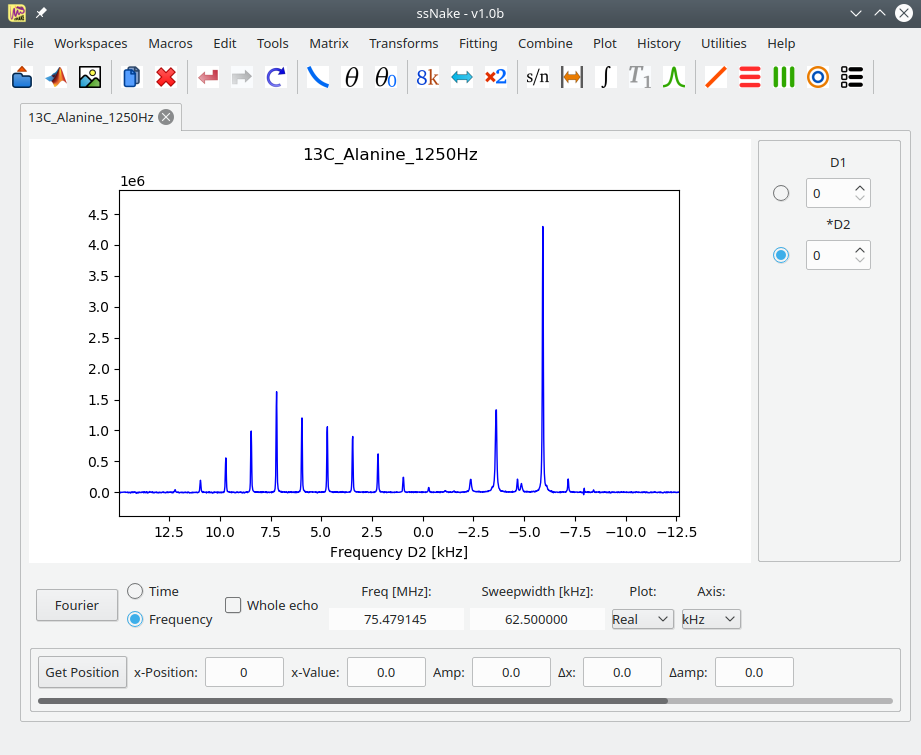
\includegraphics[width=0.8\linewidth]{Figs/Fig1.png}
\end{center}
Scrolling though D1, we can clearly see that all the sidebands change their phase, while the
centrebands of each site stay in-phase. This is the way this experiment works, and allows to
distinguish sidebands from centrebands.

We will now change the view to D1, and process this dimension.
\begin{itemize}
  \item Fill in `2438' at the D2 box in the sideframe, and press enter
\end{itemize}
This now shows the change of the centreband of this carboxyl group over the separate PASS spectra:
\begin{center}
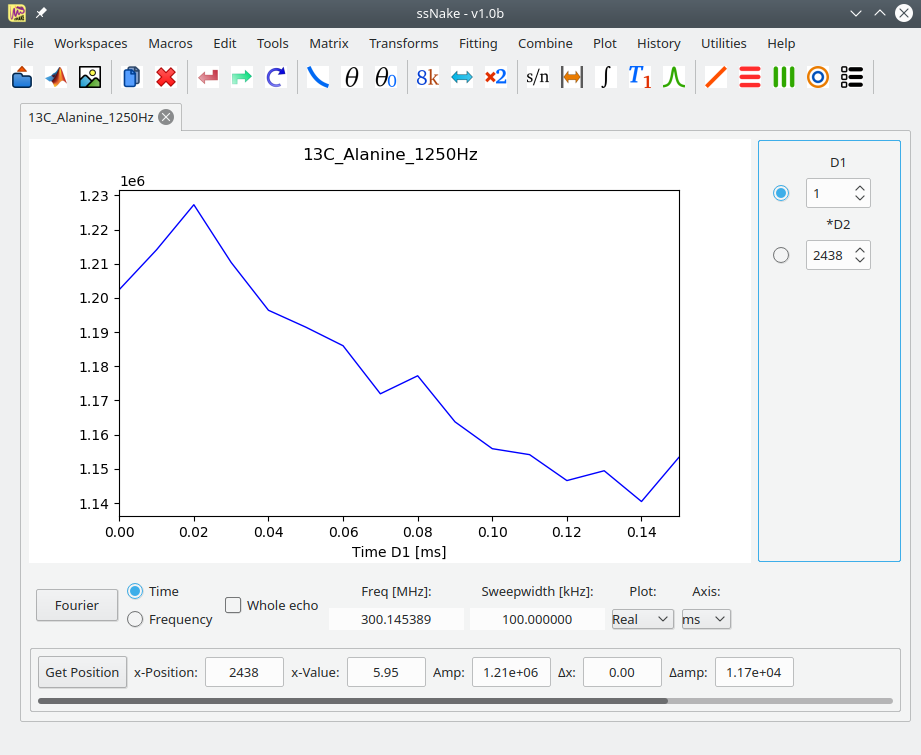
\includegraphics[width=0.8\linewidth]{Figs/Fig2.png}
\end{center}
We now want to Fourier transform also along this dimension. However, we need an extra trick. In a
regular Fourier transform, the first point of the FID is always multiplied by 0.5, to get a flat
baseline spectrum (i.e. to get rid of the frequency-independent Fourier term). This works well only
if our signal decays to 0. In the current case, we do not really have an FID, and no decay to 0 is
present. We must therefore tell ssNake to not multiply the first point by 0.5. To do this, we enable
the `Whole echo' mode in the bottom frame (tick the box).

After this, we can do transform:
\begin{itemize}
  \item Fourier transform via the `Fourier' button
  \item Clear the current ppm reference via \texttt{Tools $\longrightarrow$ Reference
	 $\longrightarrow$ Clear Current Reference}
\end{itemize}
This now shows:
\begin{center}
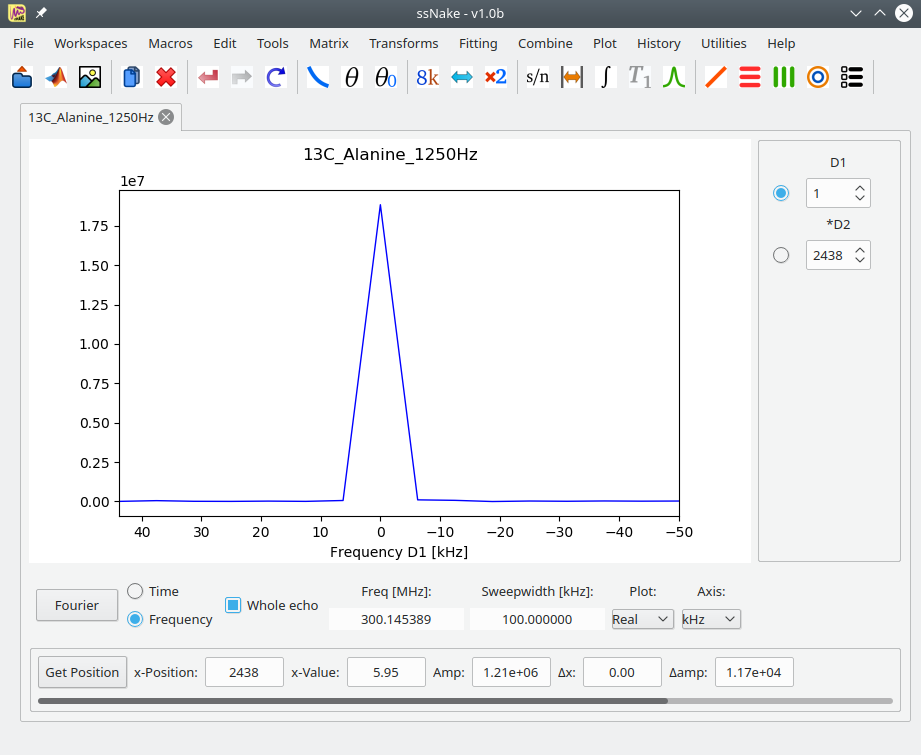
\includegraphics[width=0.8\linewidth]{Figs/Fig3.png}
\end{center}
What we see here, is that one one point has intensity: the centre point. This is exactly what we
expect here. Every point stands for a specific order of a sideband. The centrepoint is the isotropic
(order is 0) value. As our position 2438 in D2 stands for an isotropic peak, it makes sense that
only the `order is 0' point has any intensity: the sidebands are spectate.

To aid in the view of the data, we must correct the spectral width. Each point corresponds to a
specific order of sideband, so between neighboring points, there should be \SI{1250}{\Hz} difference in
frequency (i.e. the spinner frequency). In this case we have 16 points, so we must correct the
spectral width accordingly:
\begin{itemize}
  \item In the bottomframe, set the Sweepwidth to \SI{20}{\kHz} (16 * 1.250)
\end{itemize}
To have a more proper view of the data, lets view it as a contour plot:
\begin{itemize}
  \item Move to D2 by clicking its radiobutton in the sideframe
  \item Set the plot to contour via \texttt{Plot $\longrightarrow$ Contour}
\end{itemize}
This should show (zoomed):
\begin{center}
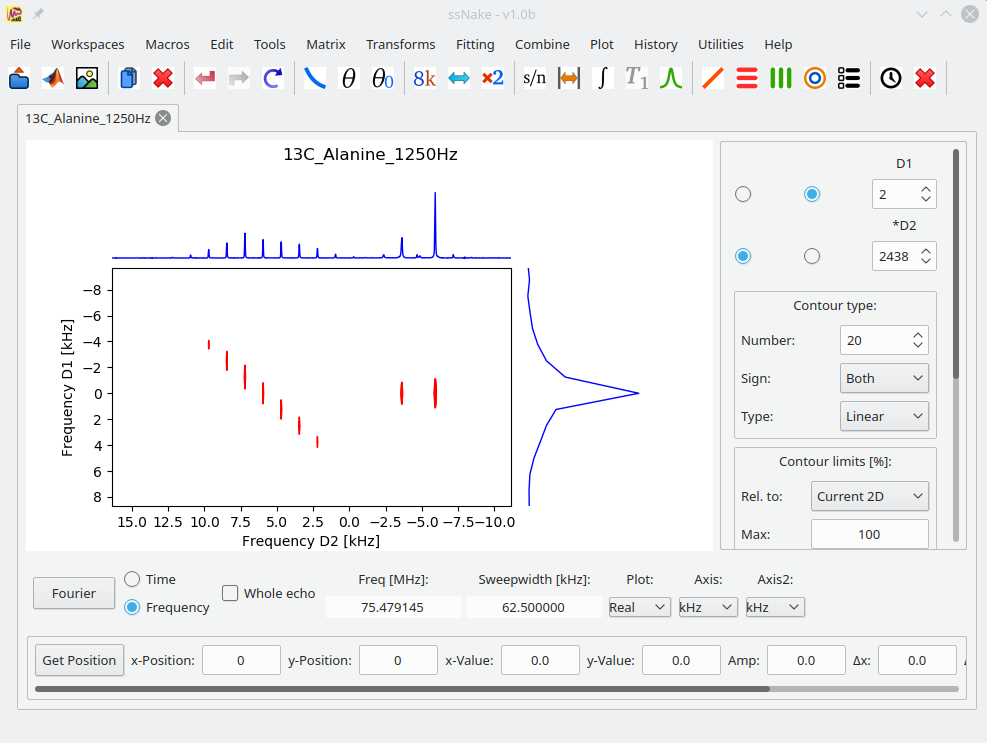
\includegraphics[width=0.8\linewidth]{Figs/Fig4.png}
\end{center}
Here we can see that the two lines on the right only have a centreband (hardly any CSA). However,
for the carboxyl group on the left, a clear pattern emerges. Every sideband is contained in a
specific trace along D1, and are therefore separated. When viewing this centreband (i.e. position 8
along D1) we will see an isotropic spectrum:
\begin{itemize}
  \item Set the plot to 1D via \texttt{Plot $\longrightarrow$ 1D Plot}
  \item Fill in `8' at the box of D1 in the side frame, and press `enter'
\end{itemize}
This should show (zoomed in):
\begin{center}
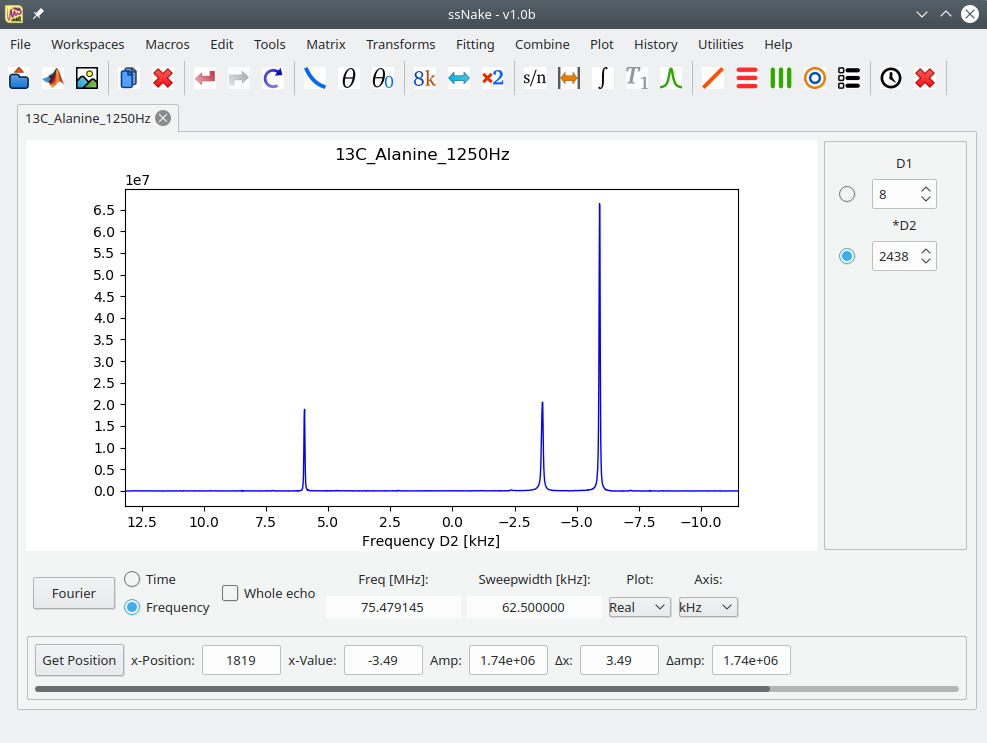
\includegraphics[width=0.8\linewidth]{Figs/Fig5.png}
\end{center}
Which is a very nice isotropic spectrum. However, by only looking at this single trace, we are
losing a lot of signal! It is therefor better to sum all the sidebands for each site. This is
actually very easy for 2D-PASS data.
\begin{itemize}
  \item Set the plot to contour via \texttt{Plot $\longrightarrow$ Contour}
\end{itemize}
Now we again have the contour plot shown above. What we will now do is shear the data in such a way
that all the sidebands of the carboxyl group end up along a vertical line along D1. As we have
\SI{1250}{\Hz} as a spinning speed, the spectrum that contains the first order sidebands much be shifted by
\SI{-1250}{\Hz} for it to align with the centreband. The same holds fro the second order sideband
(shift by $-2500$), etc. As we have corrected the spectral width of D1, we can do this via a
shearing transform.
\begin{itemize}
  \item Shear via \texttt{Matrix $\longrightarrow$ Shear} with `1' as a constant, `2' for direction,
	 and `1' for axis.
\end{itemize}
This should give:
\begin{center}
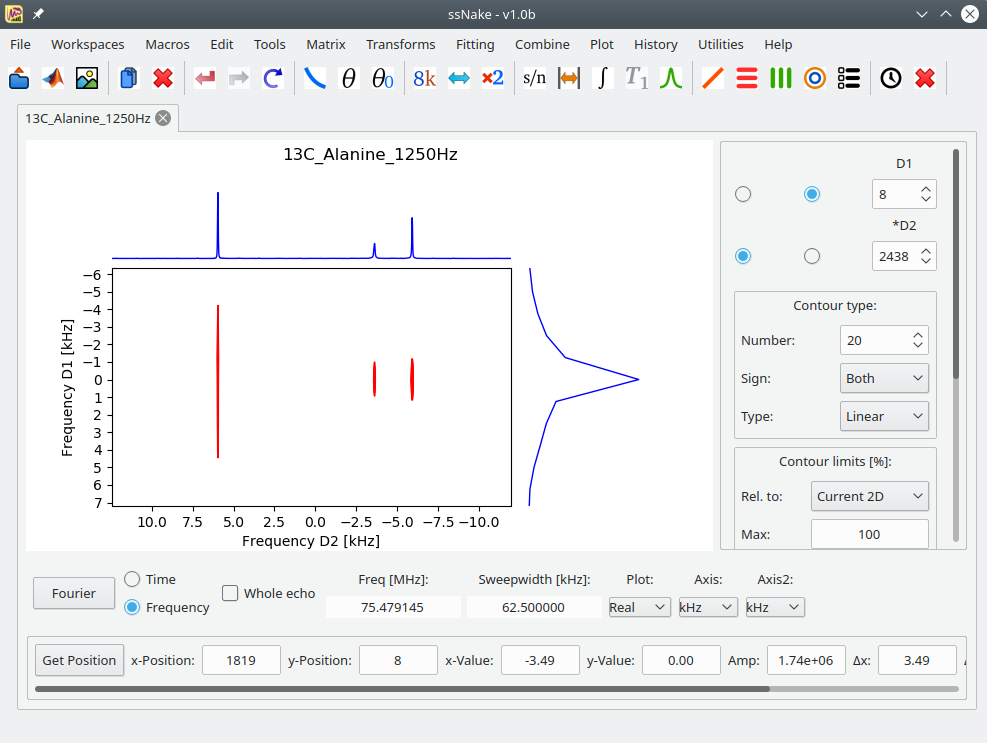
\includegraphics[width=0.8\linewidth]{Figs/Fig6.png}
\end{center}
which shows a proper alignment of the sidebands. As a final step, we will sum this data along D1:
\begin{itemize}
  \item Set the plot to 1D via \texttt{Plot $\longrightarrow$ 1D Plot}
  \item Switch to D1 using the radiobutton in the side frame
  \item Sum via \texttt{Matrix $\longrightarrow$ Region $\longrightarrow$ Sum} and push `Ok'
\end{itemize}
This shows:
\begin{center}
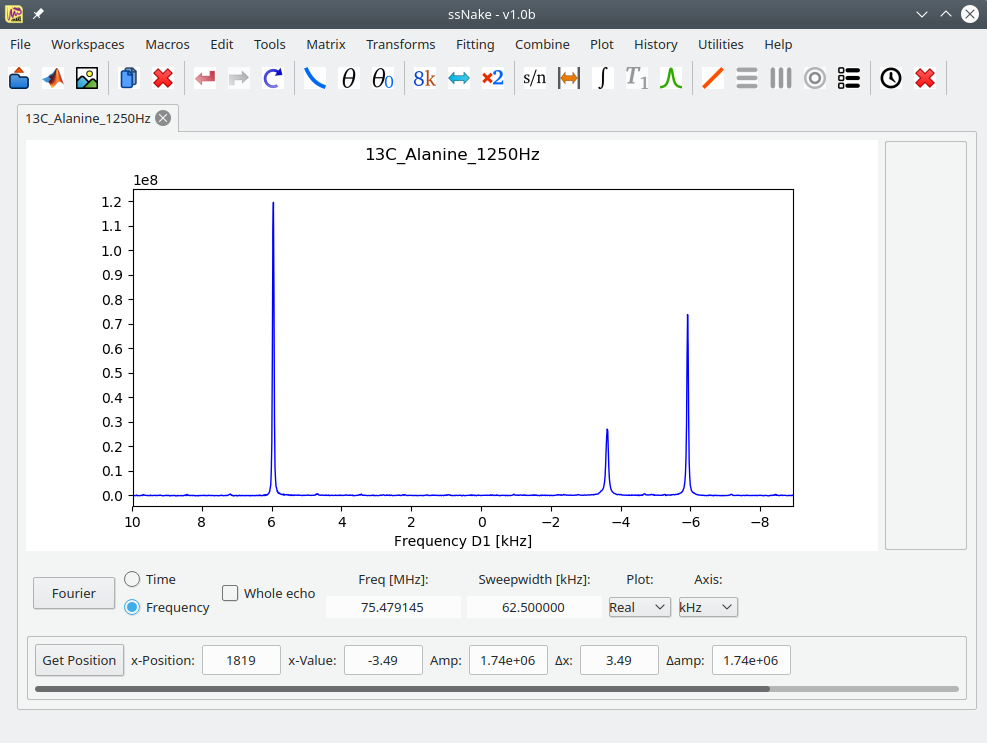
\includegraphics[width=0.8\linewidth]{Figs/Fig7.png}
\end{center}
Note that, when compared to the single trace spectrum above, the carbonyl has much more intensity in
this case (relative to the other lines). Comparing the intensities of the lines for the single trace
versus the sum tell us something about the amount of anisotropy that is present for each line.

\end{document}
